\chapter{Kimia Hijau dan Proses Industri}\label{ch:b3:green-industrial}

Ibuprofen dulu dibuat dalam enam tahap yang membuang massa lebih banyak daripada yang
dipertahankannya: garam aluminium, natrium klorida, etanol, amonia, dan asam asetat meninggalkan
pabrik untuk setiap kilogram obat. Sejak 1992, sebuah rute katalitik tiga tahap
telah mengubah sebagian besar atom yang dipakainya menjadi produk, dan satu-satunya
produk sampingnya, asam asetat, diperoleh kembali dan dijual. Bab ini memberi angka pada
perbandingan-perbandingan semacam itu: \omterm{def:b3:green-industrial:atom-economy}{ekonomi atom}, \omterm{def:b3:green-industrial:e-factor}{faktor-E}, dan \omterm{def:b3:green-industrial:pmi}{intensitas massa proses}; lalu
bab ini meninjau pelarut, energi, dan \omterm{def:b3:green-industrial:lca}{penilaian daur hidup}, bagaimana beberapa proses
kimia terbesar dibuat lebih bersih, dan apa yang diubah oleh \omterm{def:b3:green-industrial:feedstock}{bahan baku terbarukan} dan
\omterm{def:b3:complex-kinetics:enzyme}{enzim}.

\begin{recall}
Jilid sekolah memperkenalkan \omterm{def:b3:green-industrial:atom-economy}{ekonomi atom} dan \omterm{def:b3:green-industrial:green-chemistry}{kimia hijau}; Jilid Tahun 1
membahas rendemen; Jilid Tahun 2 membahas reaktor, konversi, selektivitas, waktu
tinggal, konversi sekali lewat, daur ulang dan purge, kenaikan suhu adiabatik,
elektroliser, dan sel bahan bakar. \Cref{ch:b3:surfaces-catalysis} dan
\cref{ch:b3:homogeneous-catalysis} membahas katalisis,
\cref{ch:b3:total-synthesis} ukuran-ukuran sebuah rute sintesis.
\end{recall}

\begin{omfigure}
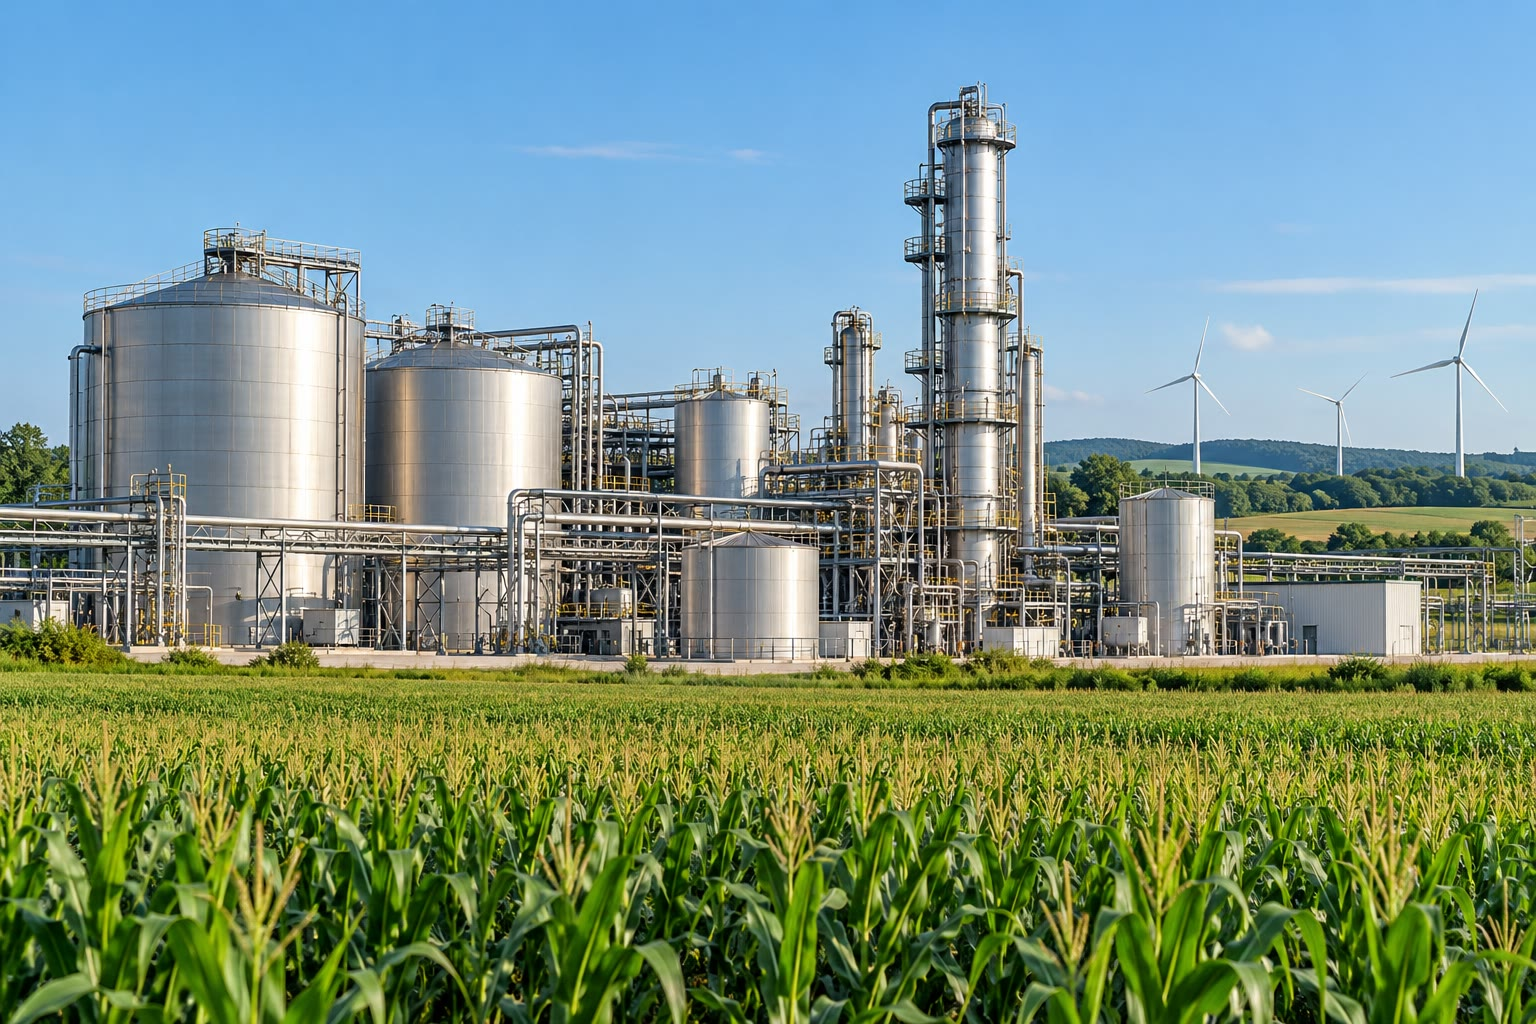
\includegraphics[width=0.58\linewidth]{images/book4/ai/b3-31-biorefinery.jpg}

{\small Sebuah biorefineri: tangki-tangki fermentasi dan kolom distilasi yang mengubah
tanaman dan residunya menjadi bahan bakar dan bahan kimia platform.}
\end{omfigure}

\section{Mengukur kehijauan}

\begin{definition}[Kimia hijau]\label{def:b3:green-industrial:green-chemistry}
Yang disebut \emph{kimia hijau}\index{kimia hijau} adalah perancangan produk
dan proses kimia yang mengurangi atau meniadakan pemakaian dan pembentukan
zat berbahaya, yang diringkas dalam dua belas asas: mencegah limbah, memaksimalkan
\omterm{def:b3:green-industrial:atom-economy}{ekonomi atom}, memakai dan membuat zat yang kurang berbahaya, merancang produk yang lebih aman,
memakai pelarut yang lebih aman, menghemat energi, memakai \omterm{def:b3:green-industrial:feedstock}{bahan baku terbarukan}, menghindari turunan
yang tidak perlu, mengutamakan katalis daripada pereaksi stoikiometrik, merancang agar mudah
terurai, memantau secara waktu nyata, dan memilih kimia yang secara inheren lebih aman.
\end{definition}

\begin{definition}[Ekonomi atom]\label{def:b3:green-industrial:atom-economy}
Yang disebut \emph{ekonomi atom}\index{ekonomi atom} sebuah reaksi adalah massa molar
produk yang dikehendaki dibagi dengan jumlah massa molar semua
pereaksi dalam persamaan setara, dalam persen.
\end{definition}

\begin{proposition}[Ekonomi atom menurut golongan reaksi]\label{prop:b3:green-industrial:ae-classes}
Reaksi adisi dan penataan ulang memiliki \omterm{def:b3:green-industrial:atom-economy}{ekonomi atom} 100\,\%; substitusi dan
eliminasi memiliki \omterm{def:b3:green-industrial:atom-economy}{ekonomi atom} yang lebih rendah.
\end{proposition}

\begin{proof}
Dalam adisi, $\mathrm{A} + \mathrm{B} \to \mathrm{AB}$, atau penataan ulang, $\mathrm{A} \to \mathrm{A'}$, satu-satunya produk memuat semua
atom pereaksi, sehingga massa molarnya sama dengan jumlah massa molar pereaksi. Sebuah
substitusi, $\mathrm{A{-}X} + \mathrm{Y} \to \mathrm{A{-}Y} + \mathrm{X}$, atau eliminasi, $\mathrm{A} \to \mathrm{B} + \mathrm{C}$, menghasilkan
produk kedua yang membawa pergi sebagian massa.
\end{proof}

\begin{definition}[Faktor-E]\label{def:b3:green-industrial:e-factor}
Yang disebut \emph{faktor-E}\index{faktor-E} sebuah proses adalah massa limbah per massa
produk. Dalam faktor-E lengkap, semua masukan yang tidak berakhir dalam produk dihitung sebagai
limbah, termasuk pelarut dan air; faktor-E sederhana tidak memasukkan pelarut dan
air.
\end{definition}

\begin{definition}[Intensitas massa proses]\label{def:b3:green-industrial:pmi}
Yang disebut \emph{intensitas massa proses}\index{intensitas massa proses} (PMI) adalah
massa total bahan yang dimasukkan ke dalam sebuah proses (pereaksi, zat pembantu, pelarut,
air) per massa produk.
\end{definition}

\begin{proposition}[PMI dan faktor-E]\label{prop:b3:green-industrial:pmi-e}
Untuk batas yang sama, $\mathrm{PMI} = E + 1$, dengan $E$ \omterm{def:b3:green-industrial:e-factor}{faktor-E} lengkap.
\end{proposition}

\begin{proof}
Menurut kekekalan massa, segala yang dimasukkan keluar sebagai produk atau sebagai limbah:
$m_{\mathrm{in}} = m_{\mathrm{product}} + m_{\mathrm{waste}}$. Pembagian dengan $m_{\mathrm{product}}$ memberikan $\mathrm{PMI} = 1 + E$.
\end{proof}

\begin{definition}[Efisiensi massa reaksi]\label{def:b3:green-industrial:rme}
Yang disebut \emph{efisiensi massa reaksi}\index{efisiensi massa reaksi} (RME) sebuah
reaksi adalah massa produk yang diperoleh dibagi dengan massa total
pereaksi yang dipakai.
\end{definition}

\begin{proposition}[RME dari rendemen dan ekonomi atom]\label{prop:b3:green-industrial:rme}
$\mathrm{RME} = \mathrm{AE} \times \text{rendemen}/\mathrm{SF}$, dengan faktor stoikiometrik $\mathrm{SF} \ge 1$ sama dengan massa
pereaksi yang dipakai dibagi dengan massa yang dituntut oleh persamaan setara.
\end{proposition}

\begin{proof}
Untuk satu mol produk yang diharapkan, persamaan itu memerlukan massa pereaksi sebesar $\sum M_r$ dan
percobaannya memakai $\mathrm{SF}\sum M_r$; percobaan itu memberikan $\text{rendemen} \times M_{\mathrm p}$ produk. Dengan membagi:
$\mathrm{RME} = \text{rendemen}\,M_{\mathrm p}/(\mathrm{SF}\sum M_r) = \mathrm{AE} \times \text{rendemen}/\mathrm{SF}$.
\end{proof}

\begin{method}[Menghitung ukuran-ukuran sebuah rute]\label{met:b3:green-industrial:metrics}
\begin{enumerate}
  \item Tuliskan persamaan setara setiap tahap dan hitunglah \omterm{def:b3:green-industrial:atom-economy}{ekonomi atom}
        rute itu dari semua pereaksi yang memasukinya.
  \item Dari catatan batch, jumlahkan massa segala yang dimasukkan (pereaksi,
        zat pembantu, pelarut, air, bahan pengerjaan): PMI = total masuk / produk.
  \item $E = \mathrm{PMI} - 1$; kurangkan aliran yang diperoleh kembali dan dipakai ulang jika aliran itu berada di dalam
        batas, dan nyatakan hal itu.
  \item RME untuk setiap tahap: produk / pereaksi, untuk menemukan di mana bahan hilang
        (rendemen rendah, pereaksi berlebih, atau \omterm{def:b3:green-industrial:atom-economy}{ekonomi atom} yang buruk).
\end{enumerate}
\end{method}

\begin{omfigure}
\begin{tikzpicture}
\begin{axis}[name=a, width=0.48\linewidth, height=5.4cm, ybar, bar width=14pt, ymin=0, ymax=110,
  xtick={1,2,3,4}, xticklabels={{ibuprofen, 6 tahap}, {ibuprofen, 3 tahap}, {EO, klorohidrin}, {EO, langsung}},
  x tick label style={font=\scriptsize, rotate=25, anchor=north east}, ylabel={ekonomi atom / \%},
  axis lines=left, tick label style={font=\scriptsize}, label style={font=\small},
  nodes near coords, nodes near coords style={font=\scriptsize, /pgf/number format/fixed, /pgf/number format/precision=0},
  enlarge x limits=0.18]
\addplot[fill=omMeth!55, draw=omMeth] table[x=i, y=AE] {figdata/out/bachelor-3-green-metrics.dat};
\end{axis}
\begin{axis}[at={(a.east)}, anchor=west, xshift=1.4cm, width=0.48\linewidth, height=5.4cm, ybar, bar width=14pt, ymin=0, ymax=3.4,
  xtick={1,2,3,4}, xticklabels={{ibuprofen, 6 tahap}, {ibuprofen, 3 tahap}, {EO, klorohidrin}, {EO, langsung}},
  x tick label style={font=\scriptsize, rotate=25, anchor=north east}, ylabel={faktor-E minimum},
  axis lines=left, tick label style={font=\scriptsize}, label style={font=\small},
  nodes near coords, nodes near coords style={font=\scriptsize, /pgf/number format/fixed, /pgf/number format/precision=2},
  enlarge x limits=0.18]
\addplot[fill=omThm!45, draw=omThm] table[x=i, y=Emin] {figdata/out/bachelor-3-green-metrics.dat};
\end{axis}
\end{tikzpicture}

{\small \omterm{def:b3:green-industrial:atom-economy}{Ekonomi atom} dua rute menuju ibuprofen dan dua rute menuju etilena oksida
(EO), serta \omterm{def:b3:green-industrial:e-factor}{faktor-E} terkecil yang dimungkinkannya (semua rendemen 100\,\%, tanpa pelarut):
$E_{\min} = (1 - \mathrm{AE})/\mathrm{AE}$. \omterm{def:b3:green-industrial:e-factor}{Faktor-E} yang sebenarnya, dengan rendemen di bawah 100\,\%, pereaksi berlebih, dan
pelarut, lebih besar.}
\end{omfigure}

\section{Pelarut dan energi}

Pelarut biasanya merupakan bagian terbesar massa sebuah proses kimia halus atau
farmasi. Pedoman pemilihan pelarut memeringkatnya berdasarkan kriteria keselamatan, kesehatan, dan
lingkungan: air, etanol, etil asetat, 2-metiltetrahidrofuran,
dan anisol direkomendasikan; diklorometana, kloroform, benzena, heksana,
dimetilformamida, dan 1,4-dioksana harus dihindari atau dilarang. Air,
karbon dioksida superkritis (yang melarutkan senyawa nonpolar dan tidak meninggalkan
residu ketika tekanannya dilepaskan), dan reaksi tanpa pelarut menyingkirkan
masalah itu dari sumbernya.

\begin{method}[Memakai pedoman pemilihan pelarut]\label{met:b3:green-industrial:solvent-choice}
\begin{enumerate}
  \item Daftarlah apa yang harus dilakukan pelarut: melarutkan pereaksi, bertahan terhadap zat pembantu,
        mendidih pada suhu yang dapat dipakai, terpisah dari air dalam pengerjaan.
  \item Pilihlah lebih dahulu dari golongan yang direkomendasikan; periksalah pernyataan bahayanya.
  \item Jika pelarut yang bermasalah diperlukan, carilah pelarut yang direkomendasikan dengan
        fungsi yang sama (2-metiltetrahidrofuran untuk diklorometana atau THF dalam
        ekstraksi, etil asetat dan heptana untuk heksana dalam kromatografi).
  \item Rencanakan perolehan kembalinya dengan distilasi, dan hitunglah bagian yang hilang dalam \omterm{def:b3:green-industrial:e-factor}{faktor-E}.
\end{enumerate}
\end{method}

\begin{definition}[Intensifikasi proses]\label{def:b3:green-industrial:intensification}
Yang disebut \emph{intensifikasi proses}\index{intensifikasi proses} adalah
perancangan ulang peralatan dan kondisi operasi agar sebuah proses menjadi jauh lebih kecil,
lebih aman, atau lebih efisien: reaktor alir kontinu dengan volume kecil dan
luas pertukaran kalor yang besar, distilasi reaktif, pemanasan gelombang mikro.
\end{definition}

Dalam reaktor alir, hanya sejumlah kecil volume zat antara berbahaya yang ada pada setiap
saat, dan kalor disingkirkan jauh lebih cepat daripada dalam bejana batch yang besar; reaksi
yang akan lepas kendali dalam tangki dapat dijalankan pada suhu dan
konsentrasi yang lebih tinggi. Katalis menggantikan pereaksi stoikiometrik, sehingga menghemat
pereaksi itu sekaligus limbah yang akan dihasilkannya: asilasi Friedel--Crafts pada rute
ibuprofen lama memakai aluminium klorida dalam jumlah stoikiometrik, yang dimusnahkan dalam
pengerjaan; rute baru memakai hidrogen fluorida sebagai katalis dan pelarut, yang
diperoleh kembali dan dipakai ulang.

\section{Pemikiran daur hidup}

\begin{definition}[Penilaian daur hidup]\label{def:b3:green-industrial:lca}
Yang disebut \emph{penilaian daur hidup}\index{penilaian daur hidup} (LCA) adalah penilaian
dampak lingkungan sebuah produk sepanjang hidupnya, dari ekstraksi bahan mentah
sampai pembuangan. Penilaian itu dinyatakan per \emph{satuan fungsional}\index{satuan fungsional},
yaitu layanan yang diberikan (misalnya, satu kali mencuci satu muatan cucian), di dalam sebuah
\emph{batas sistem}\index{batas sistem} yang menyatakan proses-proses mana yang
disertakan. Yang disebut \emph{penilaian dari buaian sampai gerbang}\index{penilaian dari buaian sampai gerbang}
berhenti ketika produk meninggalkan pabrik.
\end{definition}

\begin{omfigure}
\begin{tikzpicture}[font=\scriptsize, >=Stealth,
  box/.style={draw, rounded corners, fill=omDef!10, align=center, minimum height=8mm, inner sep=3pt}]
  \node[box] (r) at (0,0) {ekstraksi\\ bahan mentah};
  \node[box] (p) at (2.6,0) {produksi\\ kimia};
  \node[box] (f) at (5.2,0) {formulasi,\\ pengemasan};
  \node[box] (u) at (7.8,0) {pemakaian};
  \node[box] (e) at (10.2,0) {akhir hidup:\\ daur ulang,\\ pembuangan};
  \foreach \a/\b in {r/p, p/f, f/u, u/e} \draw[->, thick] (\a) -- (\b);
  \draw[omThm, thick, dashed, rounded corners] (-1.1,-0.75) rectangle (3.75,0.75);
  \node[omThm, anchor=north] at (1.3,-0.8) {batas dari buaian sampai gerbang};
  \draw[omMeth, thick, dashed, rounded corners] (-1.25,-1.35) rectangle (11.5,0.95);
  \node[omMeth, anchor=north] at (5.1,-1.4) {batas dari buaian sampai liang lahat};
  \node[anchor=south] at (5.1,1.0) {masukan: bahan, energi, air \quad keluaran: produk, emisi, limbah};
\end{tikzpicture}

{\small Tahap-tahap hidup sebuah produk dan dua \omterm{def:b3:green-industrial:lca}{batas sistem}. Masukan dan keluaran
diinventarisasi untuk setiap proses di dalam batas itu dan diubah menjadi kategori-kategori
dampak (perubahan iklim, pengasaman, pemakaian air, toksisitas\dots) yang dinyatakan per
\omterm{def:b3:green-industrial:lca}{satuan fungsional}.}
\end{omfigure}

\begin{definition}[Jejak karbon]\label{def:b3:green-industrial:carbon-footprint}
Yang disebut \emph{jejak karbon}\index{jejak karbon} sebuah produk adalah
emisi gas rumah kaca sepanjang daur hidupnya, yang dinyatakan sebagai massa karbon dioksida
dengan efek pemanasan yang sama.
\end{definition}

\begin{method}[Menyusun LCA komparatif]\label{met:b3:green-industrial:lca}
\begin{enumerate}
  \item Nyatakan tujuan dan \omterm{def:b3:green-industrial:lca}{satuan fungsionalnya}: bandingkan apa yang memberikan layanan
        yang sama, bukan massa yang sama.
  \item Gambarlah \omterm{def:b3:green-industrial:lca}{batas sistem} yang sama untuk kedua pilihan.
  \item Inventarisasikan masukan dan keluaran setiap proses di dalamnya, beserta sumber
        data dan tanggalnya.
  \item Ubahlah menjadi kategori dampak, lalu carilah kompromi-kompromi (karbon lebih rendah tetapi
        air lebih banyak) dan ujilah seberapa peka kesimpulannya terhadap data.
\end{enumerate}
\end{method}

\section{Proses-proses utama dan perbaikannya}

\begin{proposition}[Karbon dioksida dari amonia]\label{prop:b3:green-industrial:smr}
Pembuatan amonia dengan hidrogen dari reformasi kukus metana melepaskan, dari
bahan bakunya saja, $3/8$ mol $\ce{CO2}$ per mol $\ce{NH3}$: sekitar \qty{0.97}{t} $\ce{CO2}$ per ton amonia.
\end{proposition}

\begin{proof}
Reformasi yang diikuti reaksi geser air--gas secara keseluruhan adalah $\ce{CH4 + 2H2O -> CO2 + 4H2}$. Sintesisnya
adalah $\ce{N2 + 3H2 -> 2NH3}$: dua mol amonia memerlukan tiga mol hidrogen, yaitu $3/4$ mol
metana dan $3/4$ mol $\ce{CO2}$; per mol amonia, $3/8$. Satu ton amonia
(\qty{17.0}{g/mol}) adalah $\qty{5.88e4}{mol}$, yang memberikan $\qty{2.21e4}{mol} \times \qty{44.0}{g/mol} = \qty{0.97}{t}$ $\ce{CO2}$. Pembakaran metana
untuk memasok kalor reformasi menambah lebih banyak lagi.
\end{proof}

% ledger: nh3:world-2024
Pabrik-pabrik amonia, yang membuat sekitar 150 juta ton nitrogen per tahun, termasuk
sumber tunggal terbesar karbon dioksida industri; hidrogen dari
elektrolisis dengan listrik rendah karbon, atau penangkapan karbon di reformer,
adalah rute-rute untuk memangkasnya. Lingkar amonia itu sendiri, dengan konversi sekali lewatnya yang
rendah, daur ulang gas yang tidak bereaksi, dan purge argon dan metana yang
jika tidak demikian akan menumpuk, sudah efisien.

\begin{omfigure}
\begin{tikzpicture}[font=\scriptsize, >=Stealth,
  box/.style={draw, rounded corners, fill=omMeth!10, align=center, minimum height=8mm, inner sep=3pt}]
  \node[box] (m) at (0,0) {pencampur};
  \node[box] (c) at (2.6,0) {kompresor};
  \node[box] (r) at (5.2,0) {konverter\\ (katalis besi)};
  \node[box] (s) at (8.0,0) {kondensor,\\ pemisah};
  \draw[->, thick] (-1.8,0) -- (m) node[pos=0, left, align=right] {$\ce{N2 + 3H2}$\\ (umpan segar)};
  \draw[->, thick] (m) -- (c); \draw[->, thick] (c) -- (r); \draw[->, thick] (r) -- (s);
  \draw[->, thick] (s) -- ++(0,-1.2) node[below] {$\ce{NH3}$ cair};
  \draw[->, thick] (s.north) -- ++(0,0.8) -| node[pos=0.25, above] {daur ulang gas yang tidak bereaksi} (m.north);
  \draw[->, thick, omThm] ($(s.north)+(0,0.8)$) -- ++(1.6,0) node[right] {purge (Ar, $\ce{CH4}$)};
\end{tikzpicture}

{\small Lingkar sintesis amonia: gas segar dicampur dengan gas daur ulang,
dimampatkan, dan dialirkan di atas katalis; amonia diembunkan keluar, gas yang tidak bereaksi
kembali, dan aliran purge yang kecil menyingkirkan gas-gas inert yang jika tidak demikian
akan menumpuk.}
\end{omfigure}

Proses-proses besar lainnya memperlihatkan pelajaran yang sama. Proses kontak untuk asam
sulfat begitu eksotermik sehingga pabrik modern mengekspor kukus dan listrik.
Etilena oksida mula-mula dibuat melalui etilena klorohidrin, dengan kalsium
klorida sebagai limbah; oksidasi langsung etilena dengan oksigen di atas perak, sebuah
adisi dengan \omterm{def:b3:green-industrial:atom-economy}{ekonomi atom} 100\,\%, menggantikannya, dengan mengorbankan sebagian etilena yang terbakar menjadi
karbon dioksida. Propilena oksida kini juga dibuat dengan hidrogen peroksida pada
katalis \omterm{def:b3:inorganic-materials:zeolite}{zeolit} titanium, dengan air sebagai satu-satunya produk samping. Asam adipat,
yang dibuat dengan mengoksidasi sikloheksanol dan sikloheksanon dengan asam nitrat, melepaskan
dinitrogen oksida, gas rumah kaca yang kuat, yang kini dimusnahkan secara katalitik oleh pabrik-pabrik.

\section{Bahan baku terbarukan dan biokatalisis}

\begin{definition}[Bahan baku terbarukan]\label{def:b3:green-industrial:feedstock}
Yang disebut \emph{bahan baku terbarukan}\index{bahan baku terbarukan} adalah bahan mentah
yang terisi kembali dalam skala waktu manusia, seperti biomassa tumbuhan. Yang disebut \emph{molekul
platform}\index{molekul platform} adalah senyawa sederhana yang dibuat darinya dalam jumlah
besar dan diubah menjadi banyak produk: etanol, asam laktat, asam suksinat,
gliserol, asam levulinat, furfural, 5-(hidroksimetil)furfural.
\end{definition}

\begin{definition}[Biokatalisis]\label{def:b3:green-industrial:biocatalysis}
Yang disebut \emph{biokatalisis}\index{biokatalisis} adalah pemakaian \omterm{def:b3:complex-kinetics:enzyme}{enzim}, yang diisolasi atau berada di dalam
sel, sebagai katalis untuk transformasi kimia.
\end{definition}

\omterm{def:b3:complex-kinetics:enzyme}{Enzim} bekerja di dalam air di dekat suhu kamar dengan selektivitas yang luar biasa, dan
evolusi terarah kini menyesuaikannya dengan substrat-substrat yang tidak alami: sebuah transaminase
yang dievolusikan untuk tujuan itu menggantikan hidrogenasi asimetris yang dikatalisis rodium
dalam pembuatan obat diabetes sitagliptin, dan ketoreduktase membuat banyak
alkohol kiral. Karbon dioksida sendiri adalah bahan baku: urea dibuat darinya dan dari
amonia, dan metanol darinya dan dari hidrogen. Polietilena tereftalat dapat
didepolimerisasi melalui glikolisis atau metanolisis kembali menjadi monomer-monomernya, atau oleh
\omterm{def:b3:complex-kinetics:enzyme}{enzim} rekayasa, lalu dipolimerisasi ulang.

\begin{inthelab}[Mengganti diklorometana dalam pengerjaan]
Produk yang tadinya diekstraksi dari air dengan diklorometana kini diekstraksi
dengan 2-metiltetrahidrofuran: pelarut itu dibuat dari biomassa, terpisah
dengan bersih dari air (pelarut itu hanya sebagian bercampur), dan menjadi lapisan atas, bukan
lapisan bawah, sehingga urutan operasi corong pisah berubah. Lapisan-lapisan
organik dikeringkan, pelarutnya didistilasi pada tekanan rendah dan
dikumpulkan untuk dipakai ulang.
\end{inthelab}

\begin{safety}{\ghs[0.62cm]{GHS02}\ghs[0.62cm]{GHS04}\ghs[0.62cm]{GHS06}\ghs[0.62cm]{GHS08}}
% ledger: ghs4:EO, ghs:CH2Cl2, ghs4:2MeTHF
Etilena oksida: gas bertekanan yang sangat mudah menyala, beracun jika terhirup, dapat
menyebabkan kanker dan cacat genetik; zat itu hanya ada dalam sistem industri tertutup
dan unit sterilisasi. Diklorometana diduga karsinogen, dan
2-metiltetrahidrofuran mudah menyala dan korosif terhadap mata: pelarut yang lebih hijau
bukanlah pelarut yang tidak berbahaya.
\end{safety}

\begin{history}[Dua belas asas dan satu angka]
Paul Anastas dan John Warner menerbitkan dua belas asas \omterm{def:b3:green-industrial:green-chemistry}{kimia
hijau} pada 1998. Roger Sheldon memperkenalkan \omterm{def:b3:green-industrial:e-factor}{faktor-E} pada 1992, dengan mengamati bahwa
industri kimia halus dan farmasi, meskipun kecil dalam tonase,
menghasilkan jauh lebih banyak limbah per kilogram produk daripada kimia curah. Proses
ibuprofen tiga tahap, yang dimulai pada 1992, menjadi salah satu
contoh awal pendekatan baru itu.
\end{history}

\section{Latihan}

\begin{exercise}[$\star$]\label{exo:b3:green-industrial:1}
Hitunglah \omterm{def:b3:green-industrial:atom-economy}{ekonomi atom} reaksi Diels--Alder butadiena dengan etena,
esterifikasi asam asetat dengan etanol, dan reaksi Wittig
benzaldehida dengan $\ce{Ph3P=CH2}$ (yang memberikan stirena dan trifenilfosfina oksida).
\end{exercise}

\begin{exercise}[$\star$]\label{exo:b3:green-industrial:2}
Sebuah batch memakai 120 kg bahan (pereaksi, pelarut, dan air) dan memberikan 8.0 kg
produk. Hitunglah PMI dan \omterm{def:b3:green-industrial:e-factor}{faktor-E} lengkapnya.
\end{exercise}

\begin{exercise}[$\star$]\label{exo:b3:green-industrial:3}
Pilihlah \omterm{def:b3:green-industrial:lca}{satuan fungsional} untuk membandingkan dua deterjen cucian, dan jelaskan mengapa
``satu kilogram serbuk'' akan menjadi pilihan yang buruk.
\end{exercise}

\begin{exercise}[$\star$]\label{exo:b3:green-industrial:4}
Usulkan pengganti yang lebih hijau untuk diklorometana dalam ekstraksi, heksana dalam
kromatografi, dan DMF dalam kopling amida.
\end{exercise}

\begin{exercise}[$\star\star$]\label{exo:b3:green-industrial:5}
Esterifikasi 60.0 g asam asetat dengan 92.0 g etanol (dua kali
jumlah stoikiometrik) memberikan 70.4 g etil asetat. Hitunglah rendemen, \omterm{def:b3:green-industrial:atom-economy}{ekonomi
atom}, faktor stoikiometrik, dan RME, lalu periksalah hubungan di antara
keempatnya.
\end{exercise}

\begin{exercise}[$\star\star$]\label{exo:b3:green-industrial:6}
Hitunglah \omterm{def:b3:green-industrial:atom-economy}{ekonomi atom} rute klorohidrin dan rute oksidasi langsung menuju
etilena oksida, serta massa kalsium klorida yang dibuat per ton etilena oksida
oleh rute pertama.
\end{exercise}

\begin{exercise}[$\star\star$]\label{exo:b3:green-industrial:7}
Periksalah $\ce{CO2}$ per ton amonia pada bab ini, dan hitunglah $\ce{CO2}$ per ton
hidrogen yang dibuat dengan reformasi kukus.
\end{exercise}

\begin{exercise}[$\star\star$]\label{exo:b3:green-industrial:8}
Hitunglah energi listrik minimum, dalam kWh, untuk membuat satu kilogram hidrogen dengan
elektrolisis air cair pada \qty{25}{\celsius}, dari $\Delta_rG^\circ$, serta energi dari $\Delta_rH^\circ$.
\end{exercise}

\begin{exercise}[$\star\star$]\label{exo:b3:green-industrial:9}
Jika satu mol $\ce{N2O}$ terbentuk per mol asam adipat ($\ce{C6H10O4}$) dan potensi pemanasan global
$\ce{N2O}$ adalah 273 (data latihan), hitunglah $\ce{N2O}$ dan ekuivalen $\ce{CO2}$-nya
per ton asam adipat tanpa pengendalian emisi.
\end{exercise}

\begin{exercise}[$\star\star\star$]\label{exo:b3:green-industrial:10}
Tunjukkan bahwa untuk serangkaian tahap, RME keseluruhan bukan hasil kali RME
tahap-tahapnya jika pereaksi berlebih didaur ulang, dan jelaskan bagaimana daur ulang mengubah
\omterm{def:b3:green-industrial:e-factor}{faktor-E}.
\end{exercise}

\begin{exercise}[$\star\star\star$]\label{exo:b3:green-industrial:11}
Sebuah perbaikan proses memangkas pelarut dalam satu tahap dari 20 L menjadi 5 L per kilogram
produk (kerapatan pelarut \qty{0.80}{kg/L}, 90\,\% diperoleh kembali dengan distilasi, sebelum dan sesudahnya; data
latihan). Hitunglah perubahan \omterm{def:b3:green-industrial:e-factor}{faktor-E} lengkapnya.
\end{exercise}

\begin{exercise}[$\star\star\star$]\label{exo:b3:green-industrial:12}
Sebuah rute berbasis hayati menuju sebuah monomer memiliki \omterm{def:b3:green-industrial:carbon-footprint}{jejak karbon} yang lebih rendah tetapi memerlukan lebih banyak lahan
dan air daripada rute petrokimia. Bagaimana LCA komparatif akan menyajikan hal ini,
dan apa yang diperlukan untuk memutuskan di antara keduanya?
\end{exercise}

\clearpage
\enlargethispage{3\baselineskip}
\section{Soal: Ibuprofen, Enam Tahap atau Tiga?}

\begin{problem}[{Soal akhir pekan --- ibuprofen, enam tahap atau tiga: ekonomi
atom kedua rute, faktor-E-nya, katalis-katalis yang membuat
perbedaan, dan limbah yang dihindari dalam setahun}]
\label{pb:b3:green-industrial:1}
% ledger: aw:C, aw:H, aw:O, aw:Cl, aw:Na, aw:N
Data soal, per ton ibuprofen. Rute tiga tahap: 0.71 t
isobutilbenzena, 0.55 t anhidrida asetat, 0.010 t hidrogen, 0.14 t karbon
monoksida, 0.05 t pelarut dan katalis yang hilang; 0.31 t asam asetat diperoleh kembali
dan dijual. Rute enam tahap: 2.0 t pereaksi dan 1.5 t pelarut dan zat pembantu
yang tidak diperoleh kembali. Sebuah pabrik membuat 3000 t ibuprofen per tahun.

\medskip\noindent\textbf{Bagian I --- \omterm{def:b3:green-industrial:atom-economy}{Ekonomi atom}.}
\begin{enumerate}[beginpenalty=10000]
  \item Tuliskan ketiga tahap rute katalitik itu.
  \item Tuliskan persamaan keseluruhannya.
  \item Hitunglah massa-massa molar yang terlibat dan \omterm{def:b3:green-industrial:atom-economy}{ekonomi atomnya}.
  \item Daftarlah pereaksi-pereaksi rute enam tahap (asilasi Friedel--Crafts, kondensasi
        Darzens dengan etil kloroasetat dan natrium etoksida, hidrolisis dan
        dekarboksilasi, pembentukan oksim, dehidrasi menjadi nitril, hidrolisis).
  \item Hitunglah \omterm{def:b3:green-industrial:atom-economy}{ekonomi atomnya} dari jumlah massa molar pereaksi-pereaksi itu (dengan dua
        molekul air).
  \item Produk samping apakah yang meninggalkan rute lama?
\end{enumerate}

\medskip\noindent\textbf{Bagian II --- \omterm{def:b3:green-industrial:e-factor}{Faktor-E}.}
\begin{enumerate}[resume, beginpenalty=10000]
  \item Hitunglah massa yang dimasukkan ke dalam rute baru per ton produk.
  \item Hitunglah PMI dan \omterm{def:b3:green-industrial:e-factor}{faktor-E} lengkapnya, dengan asam asetat dihitung sebagai limbah.
  \item Hitunglah \omterm{def:b3:green-industrial:e-factor}{faktor-E} jika asam asetat yang diperoleh kembali dihitung sebagai produk.
  \item Hitunglah PMI dan \omterm{def:b3:green-industrial:e-factor}{faktor-E} rute lama.
  \item Mengapa \omterm{def:b3:green-industrial:e-factor}{faktor-E} yang sebenarnya lebih besar daripada $(1 - \mathrm{AE})/\mathrm{AE}$?
  \item Asas-asas manakah dari kedua belas asas itu yang diilustrasikan oleh perbedaan itu?
\end{enumerate}

\medskip\noindent\textbf{Bagian III --- Katalis.}
\begin{enumerate}[resume, beginpenalty=10000]
  \item Apakah yang digantikan hidrogen fluorida dalam asilasi, dan mengapa hal itu penting?
  \item Apakah yang mengkatalisis hidrogenasi keton menjadi alkohol?
  \item Apakah yang mengkatalisis \omterm{def:b3:homogeneous-catalysis:carbonylation}{karbonilasi} alkohol, dan kimia bab manakah itu?
  \item Mengapa asam asetat menjadi produk samping pada kedua rute?
  \item Bahaya apakah yang dibawa rute baru, dan bagaimana bahaya itu dikelola?
  \item Mengapa tahap yang lebih sedikit juga berarti energi yang lebih sedikit?
\end{enumerate}

\medskip\noindent\textbf{Bagian IV --- Setahun.}
\begin{enumerate}[resume, beginpenalty=10000]
  \item Hitunglah limbah rute lama untuk keluaran tahunan pabrik itu.
  \item Hitunglah limbah rute baru (asam asetat dijual).
  \item Hitunglah limbah yang dihindari per tahun.
  \item Apakah \omterm{def:b3:green-industrial:e-factor}{faktor-E} yang lebih rendah selalu berarti dampak lingkungan yang lebih rendah?
  \item Apakah yang akan ditambahkan oleh sebuah \omterm{def:b3:green-industrial:lca}{penilaian daur hidup}?
  \item Nyatakan hasilnya: \omterm{def:b3:green-industrial:atom-economy}{ekonomi atom} rute tiga tahap.
\end{enumerate}
\end{problem}
